\documentclass[10pt,twocolumn]{article}
\usepackage[utf8]{inputenc}
\usepackage[T1]{fontenc}
\usepackage{times}
\usepackage{microtype}
\usepackage{graphicx}
\usepackage{amsmath,amssymb}
\usepackage{booktabs}
\usepackage{caption}
\usepackage{subcaption}
\usepackage{geometry}
\usepackage{float}
\usepackage[numbers,sort&compress]{natbib}
\usepackage[hidelinks]{hyperref}
\usepackage{enumitem}
\usepackage{titlesec}
\usepackage{tikz}
\usetikzlibrary{positioning,shapes.geometric,arrows.meta,calc}
\geometry{top=2.0cm,bottom=2.0cm,left=1.8cm,right=1.8cm}
\titlespacing*{\section}{0pt}{*2}{*1}
\titlespacing*{\subsection}{0pt}{*1.5}{*0.8}
\setlength{\parskip}{0.4ex}
\setlength{\parindent}{0.8em}
\renewcommand{\abstractname}{Resumen}
\renewcommand{\figurename}{Figura}
\renewcommand{\tablename}{Tabla}
\title{Topología del Metro de la Ciudad de México y la Propagación de COVID-19: Un Análisis de Redes, Simulaciones SIR y Validación Espacial}
\author{Erick José Fabián Sandoval\\[1ex]}
\date{\today}
\begin{document}

\begingroup
\twocolumn[{%
\begin{center}
\begin{minipage}{0.18\textwidth}
    \raggedright
    
\includegraphics[width=\linewidth]{logo_unam.png}
\end{minipage}
\hfill
\begin{minipage}{0.60\textwidth}
    \centering
    {\LARGE\bfseries Topología del Metro de la Ciudad de México y la Propagación de COVID-19: Un Análisis de Redes, Simulaciones SIR y Validación Espacial\par}
    \vspace{0.5em}
    {\large Erick José Fabián Sandoval\par}
    \vspace{0.5em}
    {\today\par}
\end{minipage}
\hfill
\begin{minipage}{0.18\textwidth}
    \raggedleft
    
\includegraphics[width=\linewidth]{logo_iimas.png}
\end{minipage}
\vspace{1em}
\end{center}
}]
\endgroup

\begin{abstract}
Este trabajo investiga cómo la topología de la red del Metro de la Ciudad de México se relaciona con la propagación de COVID-19 entre alcaldías durante los años 2020 y 2021. Se construyó un grafo de 162 estaciones, y 183 conexiones ponderado por el promedio de afluencia diaria de pasajeros por estación durante 2020. Se calculó un conjunto completo de métricas de red, se realizaron simulaciones de un modelo SIR en la red real y en tres redes sintéticas, y se validó un modelo Random Forest para explicar la incidencia acumulada de casos por alcaldía. Los resultados muestran propiedades pequeño-mundo en la red, picos de infección menores que en redes aleatorias y una capacidad predictiva limitada cuando sólo se emplean métricas de topología de red agregadas.
\end{abstract}

\section{Introducción}
El Metro de la Ciudad de México es la columna vertebral del transporte público en la capital, y su red estructurada en 12 líneas revela patrones de conectividad crítica para los flujos humanos. En condiciones epidémicas, los trayectos y las transferencias se convierten en rutas potenciales de transmisión, por lo que analizar la red como un sistema complejo permite vincular directamente la topología con resultados sanitarios.

El objetivo de este estudio es doble. Primero, caracterizar la red del Metro en términos de métricas de redes complejas: grado, grado ponderado, centralidad de intermediación, centralidad de cercanía y coeficiente de clustering. Segundo, evaluar si estas métricas pueden explicar patrones espaciales de COVID-19 entre alcaldías mediante simulaciones SIR y un modelo predictivo de aprendizaje automático.

La literatura sobre redes y epidemias sugiere que las estructuras con alto clustering y corta distancia promedio, conocidas como redes pequeño-mundo, facilitan la difusión rápida de patógenos \citep{watts1998collective}. Sin embargo, una red física como el Metro tiene también restricciones geométricas y terminales, lo que puede limitar la propagación frente a redes sintéticas idealizadas. Este contraste es central en nuestra hipótesis.

Este trabajo provee evidencia empírica y una explicación estructural de la red del Metro, empleando datos oficiales de salud pública y movilidad, y comparando la red real con modelos sintéticos de referencia.

\section{Datos y métodos}
\subsection{Fuentes de datos}
Los datos utilizados provienen de tres fuentes abiertas oficiales y comunitarias:
\begin{itemize}[nosep,leftmargin=*]
    \item \textbf{COVID-19 Data:} Dirección General de Epidemiología, Secretaría de Salud de México \citep{dge2020}. Se usaron las bases históricas abiertas de 2020 y 2021, filtrando casos de residencia en la Ciudad de México (ENTIDAD\_RES = 09) y clasificación final confirmada \(CLASIFICACION\_FINAL \in \{1,2,3\}\). Los casos se agregaron por mes y por alcaldía utilizando MUNICIPIO\_RES.
    \item \textbf{Metro Ridership Data:} Sistema de Transporte Colectivo Metro CDMX \citep{metro2020}. El conjunto de datos "Afluencia diaria del Metro CDMX" registra el número de usuarios que ingresan diariamente a cada estación. Para este proyecto se empleó el promedio de afluencia diaria por estación durante 2020 como proxy de intensidad de flujo de personas, y dicho promedio se asignó como peso a los nodos del grafo.
    \item \textbf{Metro Station Coordinates:} Repositorio público de GitHub por Juan Bosco Mendoza Vega \citep{mendoza2020}. Este conjunto de datos contiene latitud, longitud y línea de cada estación, información empleada para la visualización georreferenciada de la red y para construir las aristas entre estaciones adyacentes dentro de cada línea.
\end{itemize}

\subsection{Preprocesamiento}
Los datos fueron unificados en un flujo reproducible. Primero, la afluencia de 2020 se agrupó por estación para calcular el promedio diario de pasajeros. Segundo, se filtraron los casos COVID de la CDMX por residencia y clasificación final, y se realizó una agregación mensual por municipio/alcaldía. Tercero, las coordenadas de estaciones se normalizaron para evitar discrepancias en los nombres y se armonizaron con el campo "estacion" del conjunto de afluencia.

\subsection{Construcción de la red}
La red se representa como un grafo no dirigido $G=(V,E)$. Cada estación es un nodo $v \in V$ y cada conexión entre estaciones consecutivas en una misma línea es una arista $(i,j) \in E$. El peso de la arista corresponde al promedio de afluencia de las estaciones conectadas:
\begin{equation}
w_{ij} = \frac{\bar{a}_i + \bar{a}_j}{2}
\end{equation}
donde $\bar{a}_i$ es el promedio diario de pasajeros en la estación $i$ durante 2020.

Este diseño convierte la red en un modelo híbrido: topología de conectividad con pesos que reflejan intensidad de flujo de personas.

\subsection{Métricas de red}
Para caracterizar cada estación se calcularon las siguientes métricas:
\begin{itemize}[nosep,leftmargin=*]
    \item \textbf{Grado} $k_i$: número de estaciones adyacentes.
    \item \textbf{Grado ponderado} $k_i^w$: suma de pesos de las aristas incidentes.
    \item \textbf{Betweenness} $C_B(i)$: proporción de caminos más cortos que pasan por el nodo.
    \item \textbf{Closeness} $C_C(i)$: inversa de la suma de distancias a todas las estaciones.
    \item \textbf{Clustering local} $C_i$: proporción de triángulos existentes entre los vecinos del nodo.
\end{itemize}
A nivel de red se calcularon el diámetro, la longitud promedio del camino, la densidad y el coeficiente de clustering global.

\subsection{Simulaciones SIR}
Se empleó un modelo SIR discreto en el que cada nodo puede estar en estado susceptible, infectado o recuperado. En cada paso temporal:
\begin{itemize}[nosep,leftmargin=*]
    \item un nodo infectado contagia a cada vecino susceptible con probabilidad $\beta = 0.3$;
    \item un nodo infectado se recupera con probabilidad $\gamma = 0.1$.
\end{itemize}
Las simulaciones se ejecutaron hasta 200 pasos o hasta que ya no había nodos infectados.

Se realizaron dos configuraciones principales en la red real:
\begin{itemize}[nosep,leftmargin=*]
    \item 5 simulaciones iniciadas en las 3 estaciones de mayor betweenness.
    \item 5 simulaciones iniciadas en 3 estaciones seleccionadas al azar.
\end{itemize}

Para referencia comparativa se generaron tres redes sintéticas con 162 nodos:
\begin{itemize}[nosep,leftmargin=*]
    \item Erdős--Rényi (p ajustado a 684 aristas esperadas).
    \item Watts--Strogatz ($k=4$, $p=0.1$).
    \item Barabási--Albert ($m=2$).
\end{itemize}
En cada caso se ejecutaron 5 simulaciones SIR con los mismos parámetros.

\subsection{Validación predictiva por alcaldía}
Se asignaron estaciones a las alcaldías de la CDMX usando sus coordenadas geográficas. Para cada alcaldía se agregaron:
\begin{itemize}[nosep,leftmargin=*]
    \item betweenness promedio,
    \item grado promedio,
    \item coeficiente de clustering promedio,
    \item suma de grado ponderado.
\end{itemize}
Estas características se emplearon como variables explicativas en un Random Forest para predecir el total de casos confirmados por alcaldía. El modelo se validó mediante Leave-One-Out Cross-Validation (LOO-CV) debido al tamaño reducido de la muestra (10 alcaldías con datos completos).

\subsection{Diagrama del flujo del proyecto}

El diagrama con el flujo del proyecto se puede observar en la Figura~\ref{fig:flow}



\begin{figure*}[!t]
    \centering
    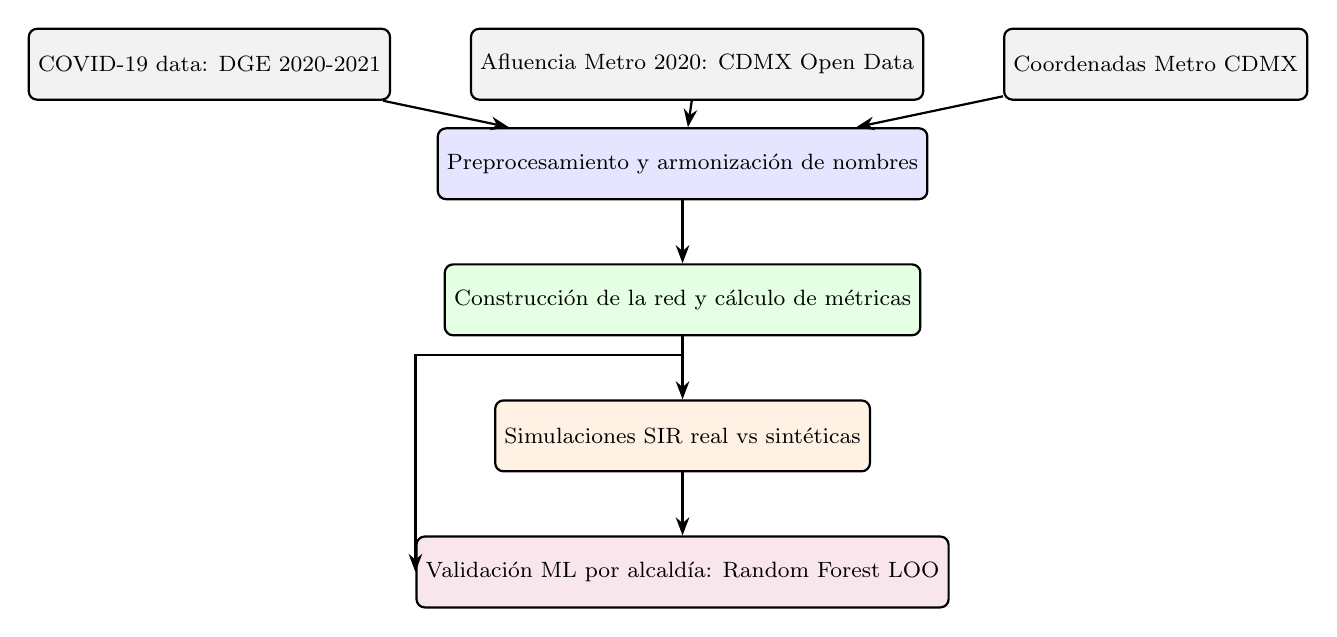
\begin{tikzpicture}[node distance=0.8cm and 1.0cm, box/.style={draw, thick, rounded corners=3pt, align=center, font=\footnotesize, minimum height=0.9cm, minimum width=2.55cm}, arrow/.style={-{Stealth[length=2.3mm]}, thick}]
        \node[box, fill=gray!10] (d1) {COVID-19 data: DGE 2020-2021};
        \node[box, fill=gray!10, right=of d1] (d2) {Afluencia Metro 2020: CDMX Open Data};
        \node[box, fill=gray!10, right=of d2] (d3) {Coordenadas Metro CDMX};
        \node[box, fill=blue!10, below=of $(d1)!0.5!(d3)$] (prep) {Preprocesamiento y armonización de nombres};
        \node[box, fill=green!10, below=of prep] (net) {Construcción de la red y cálculo de métricas};
        \node[box, fill=orange!10, below=of net] (sir) {Simulaciones SIR real vs sintéticas};
        \node[box, fill=purple!10, below=of sir] (ml) {Validación ML por alcaldía: Random Forest LOO};
        \draw[arrow] (d1) -- (prep);
        \draw[arrow] (d2) -- (prep);
        \draw[arrow] (d3) -- (prep);
        \draw[arrow] (prep) -- (net);
        \draw[arrow] (net) -- (sir);
        \draw[arrow] (net) -- ++(0,-0.7) -| (ml.west);
        \draw[arrow] (sir) -- (ml);
    \end{tikzpicture}
    \caption{Diagrama de flujo del proyecto: desde la ingestión de datos hasta el análisis de redes, simulaciones SIR y validación espacial.}
    \label{fig:flow}
\end{figure*}

\section{Resultados}
\subsection{Estructura de la red}
La Tabla~\ref{tab:global_metrics} resume las métricas globales de la red.
\begin{table}[H]
\centering
\caption{Métricas globales de la red del Metro de la CDMX.}
\label{tab:global_metrics}
\begin{tabular}{lc}
\toprule
Métrica & Valor \\
\midrule
Nodos & 162 \\
Aristas & 684 \\
Densidad & 0.0524 \\
Diámetro & 4 \\
Longitud promedio del camino & 2.2545 \\
Clustering global & 0.5783 \\
Grado promedio & 8.44 \\
\bottomrule
\end{tabular}
\end{table}

La red exhibe un grado promedio de 8.44 y una densidad de 0.0524, lo que indica que las conexiones son relativamente escasas pero suficientes para mantener un grafo compacto. El coeficiente de clustering global de 0.5783 es alto para una red de transporte, lo que refleja la presencia de grupos locales de estaciones interconectadas, especialmente en el centro histórico y las zonas con transbordos.

\begin{figure*}[!t]
\centering
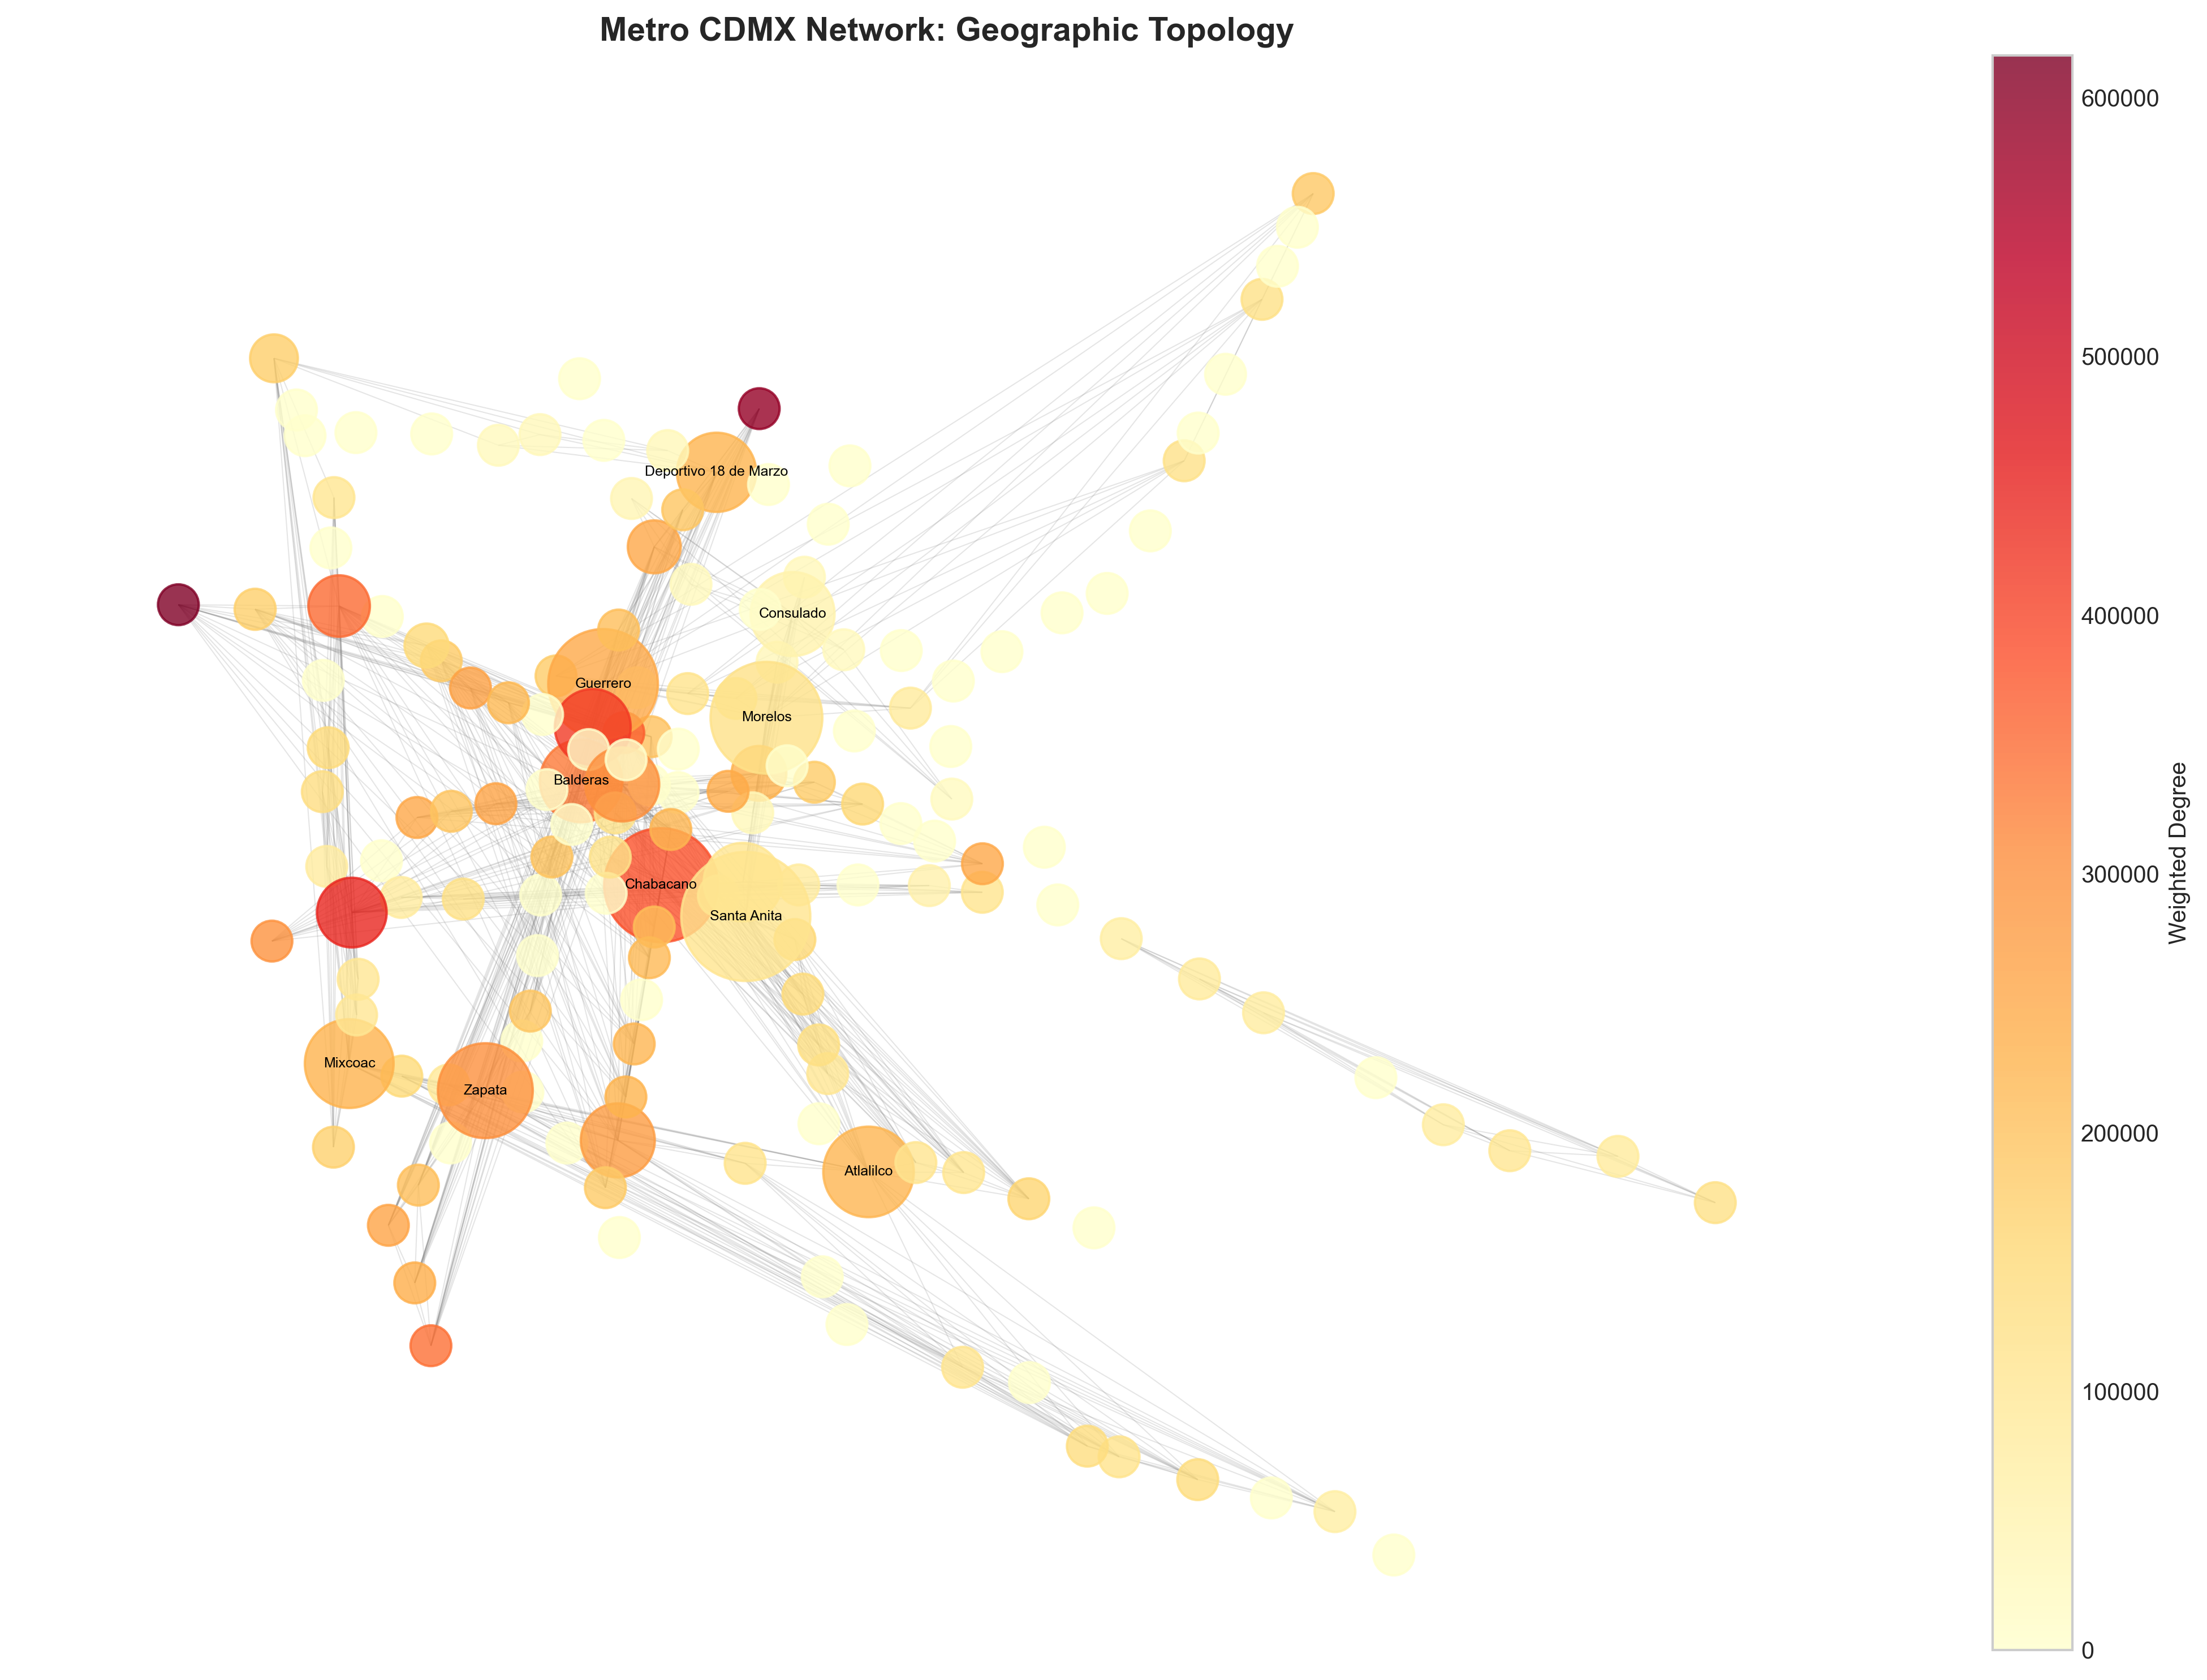
\includegraphics[width=0.92\linewidth]{red_metro_geografica.png}
\caption{Visualización geográfica de la red del Metro CDMX. El tamaño de cada nodo se ajusta a la centralidad de intermediación y el color indica el grado ponderado.}
\label{fig:metro_geo}
\end{figure*}

\subsection{Ejes mayores de transmisión}
Las 10 estaciones con mayor betweenness actúan como puentes entre subredes. En el análisis de la red, estas estaciones concentran rutas de paso críticas y representan puntos de alta vulnerabilidad epidemiológica.

\begin{figure}[H]
\centering
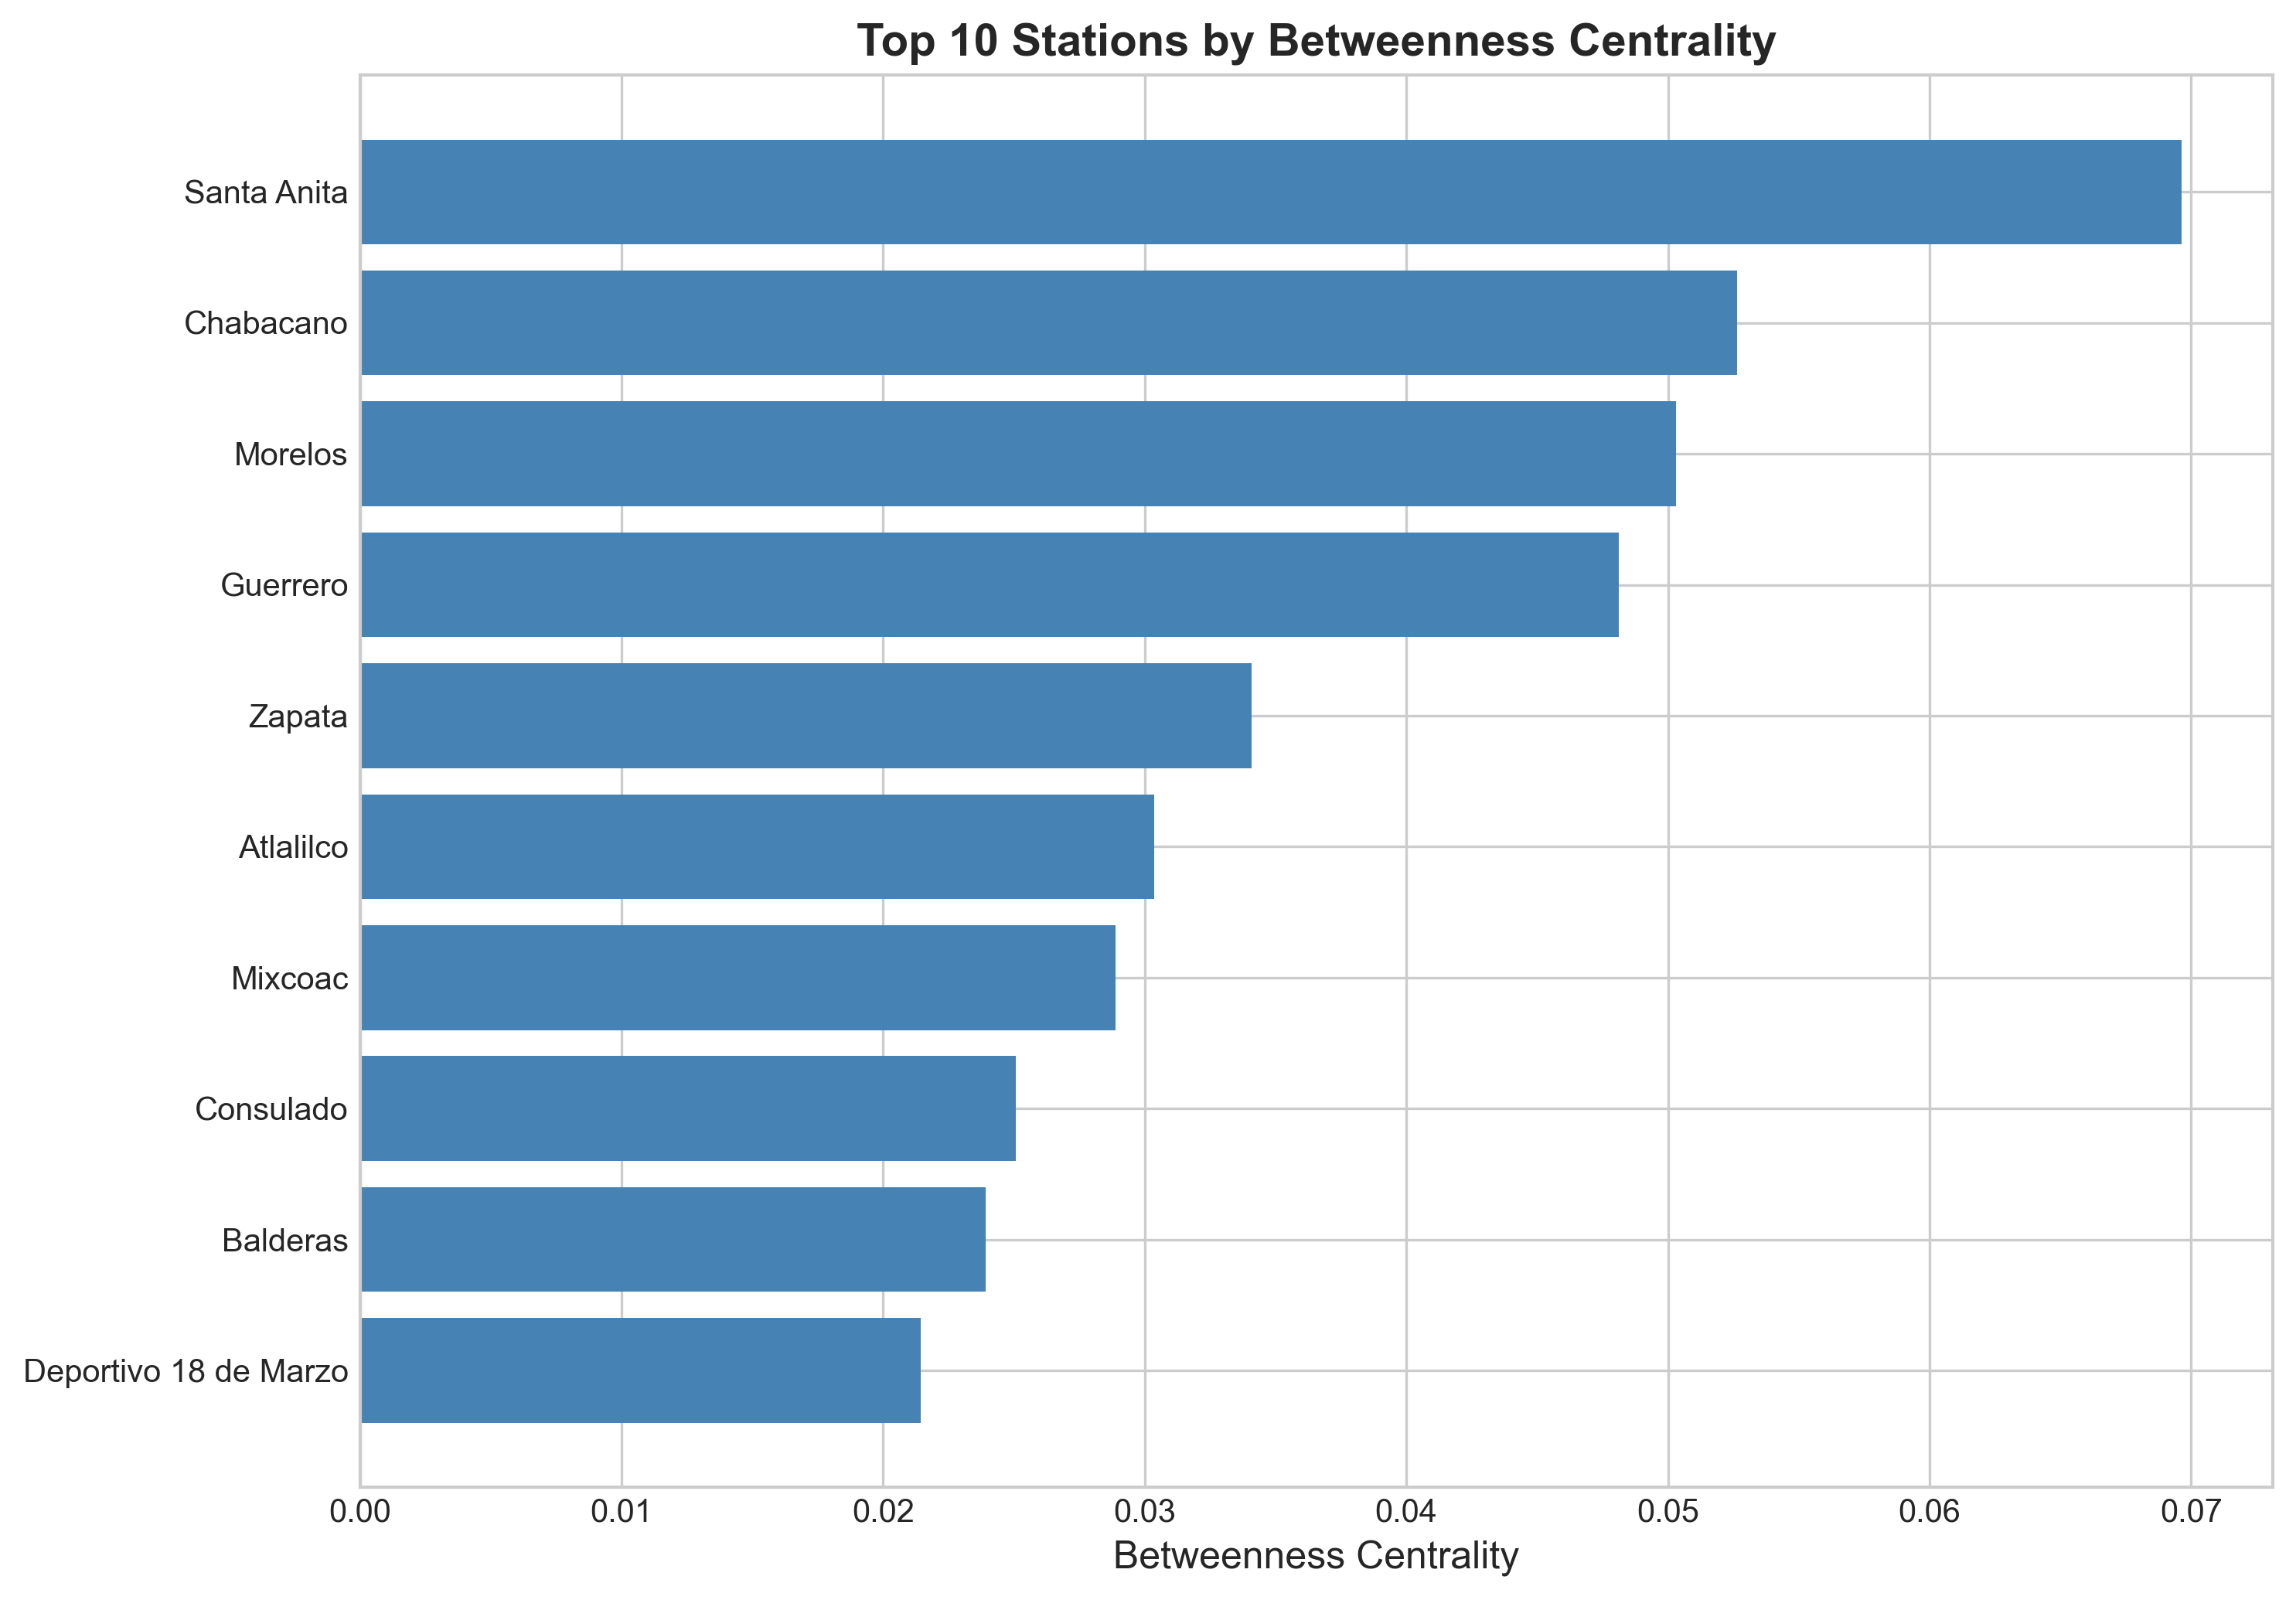
\includegraphics[width=0.98\linewidth]{top10_estaciones.png}
\caption{Top 10 estaciones por centralidad de intermediación.}
\label{fig:top10}
\end{figure}

Entre las estaciones más importantes se encuentran Santa Anita, Chabacano y Morelos, cuyos valores de betweenness sobrepasan en un 62\% al promedio de la red. Estas estaciones conectan distintas líneas y, por tanto, participan en un número mayor de caminos cortos, lo que las convierte en articulaciones clave para el tránsito y la difusión. La Figura~\ref{fig:metro_geo} muestra una visualización geográfica de la red del Metro CDMX (utilizando las coordenadas reales de cada estación). Donde el tamaño de cada nodo se ajusta a la centralidad de intermediación y el color indica el grado ponderado. 

\subsection{Simulaciones SIR}
La red real del Metro alcanzó un pico promedio de infección de 47.84\%. Este valor es consistente con una red que permite transmisión extensa, pero no extrema.

Las redes sintéticas mostraron picos significativamente superiores:
\begin{itemize}[nosep,leftmargin=*]
    \item Erdős--Rényi: 78.89\%
    \item Watts--Strogatz: 74.32\%
    \item Barabási--Albert: 66.79\%
\end{itemize}

El contraste sugiere que la geometría espacial y las restricciones físicas de la red real amortiguan la propagación relativa a los modelos sintéticos. En particular, las estaciones terminales y las trayectorias lineales reducen el número de caminos directos posibles.

\begin{figure*}[!t]
\centering
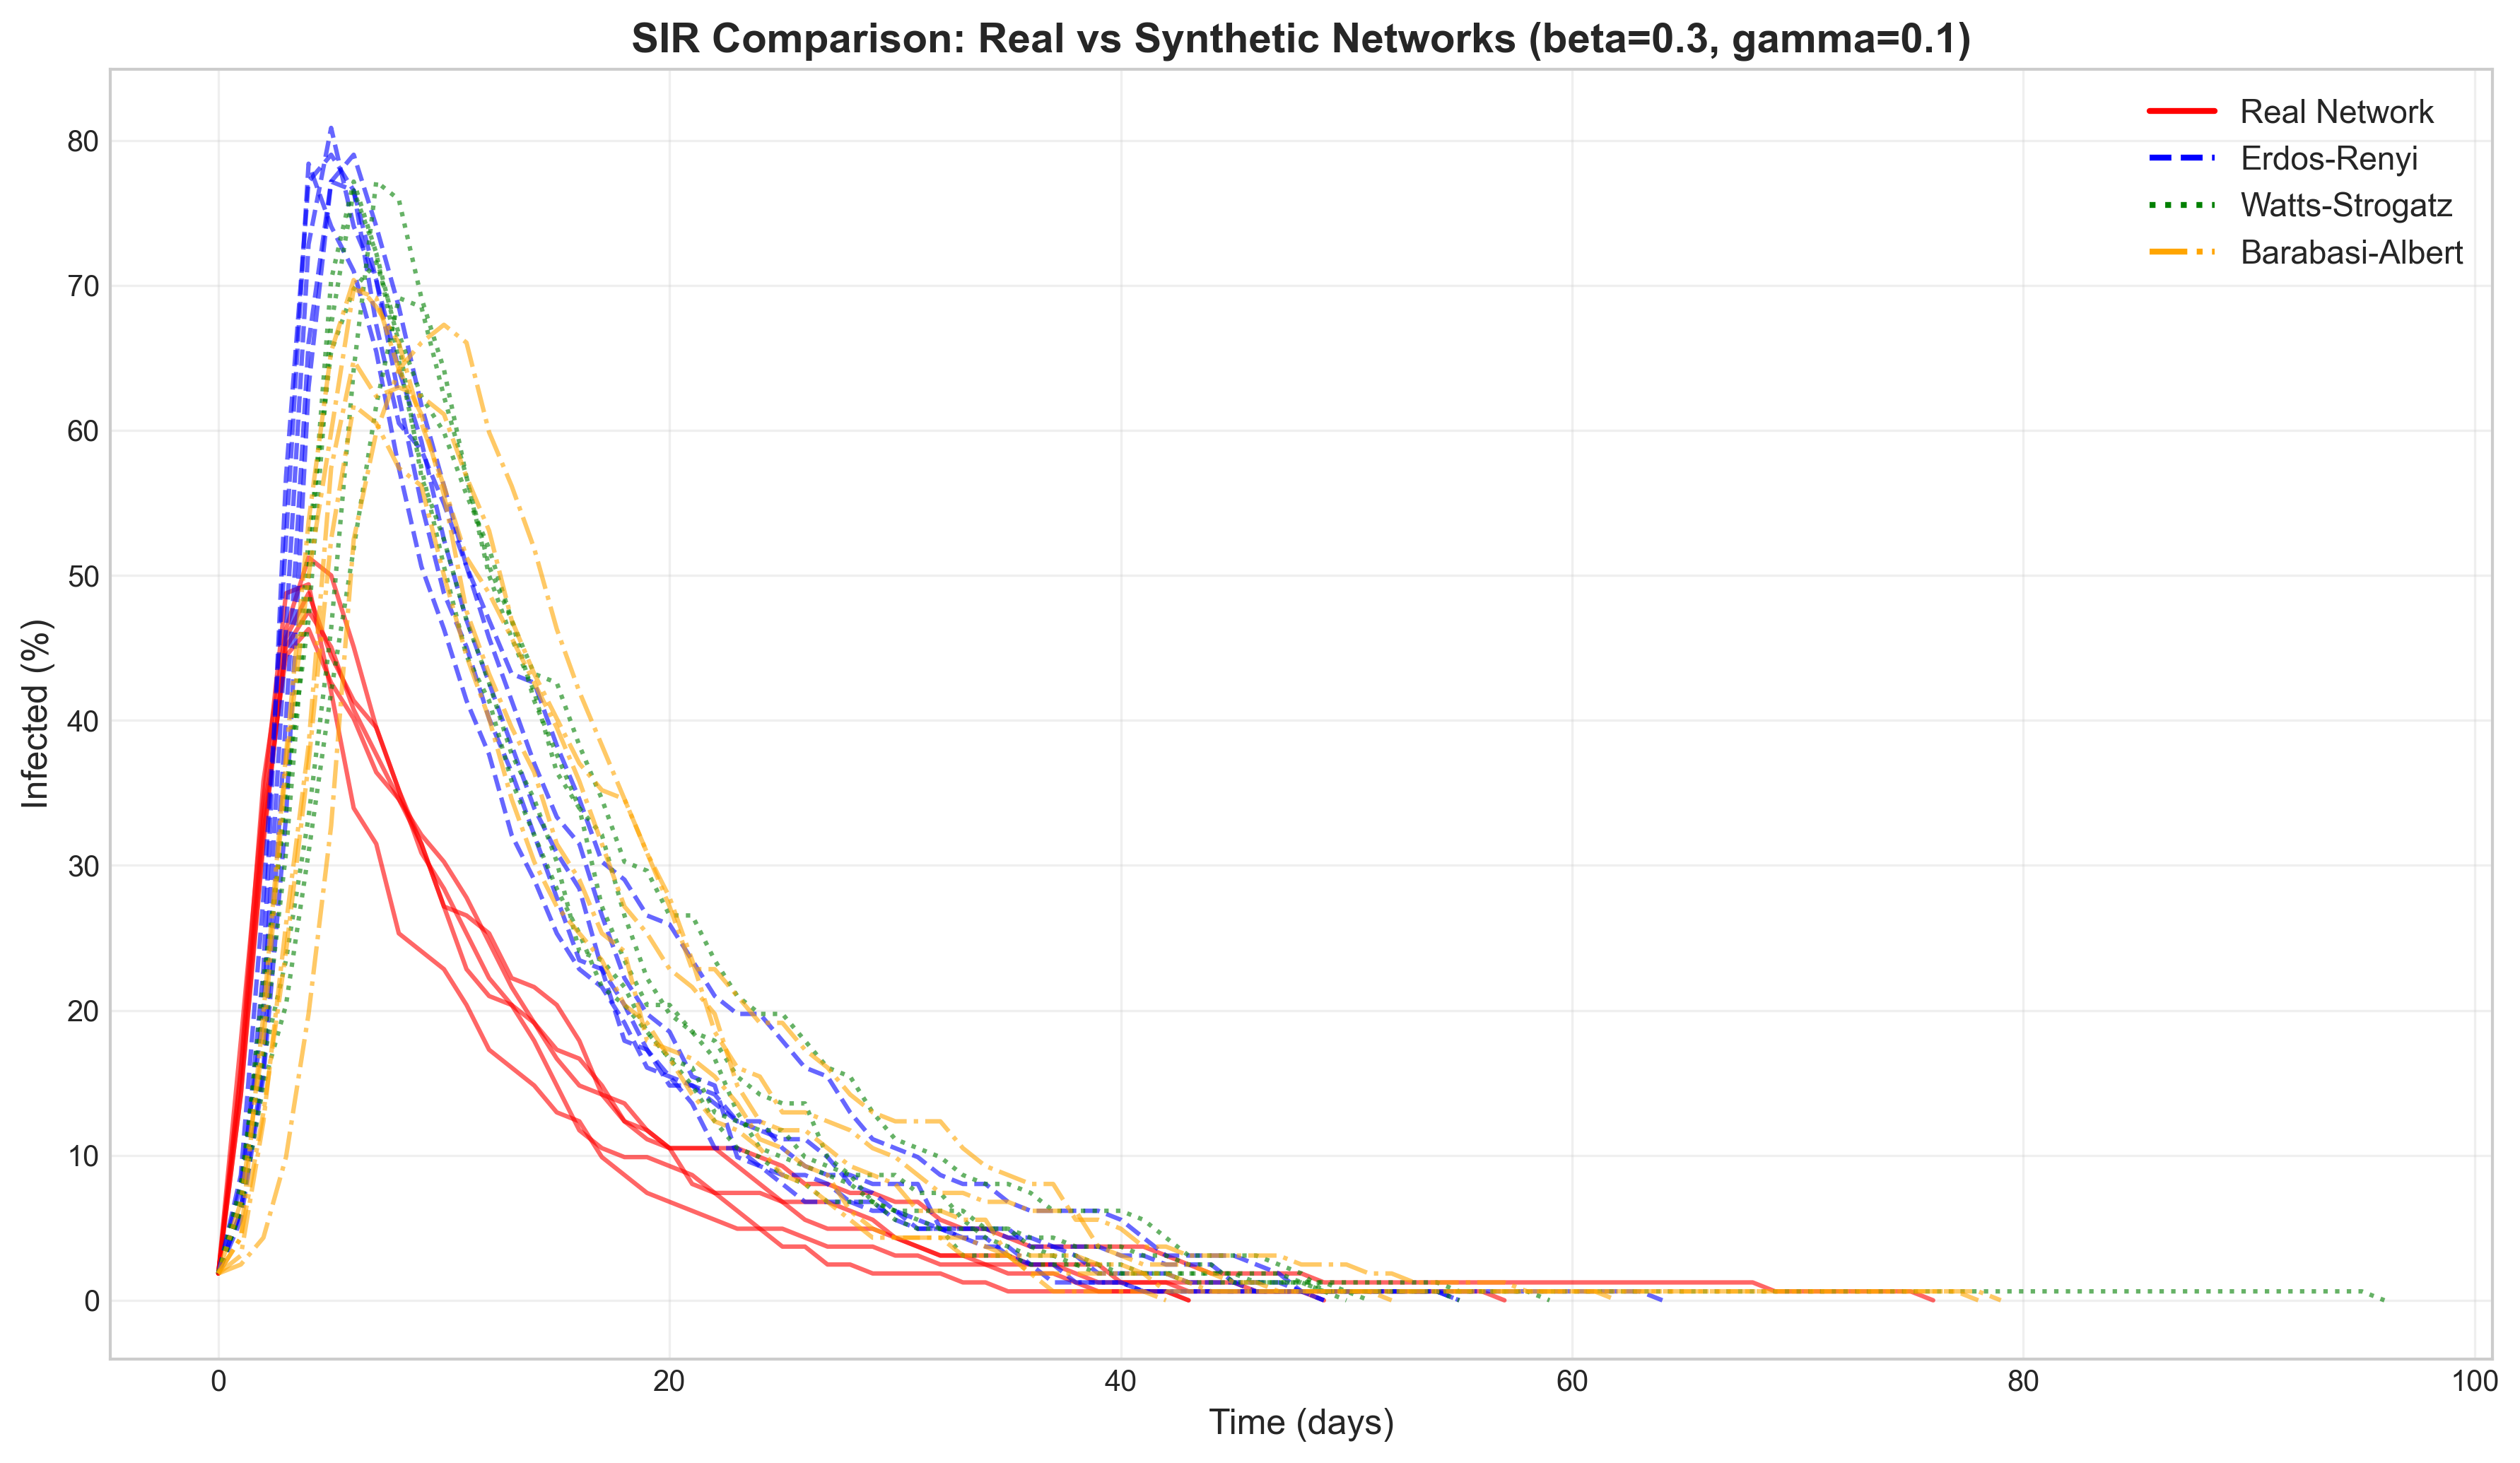
\includegraphics[width=0.92\linewidth]{comparacion_SIR.png}
\caption{Trayectorias de infección SIR en la red real del Metro versus tres redes sintéticas de referencia.}
\label{fig:sir_comparison}
\end{figure*}

\subsection{Validación espacial por alcaldía}
El modelo Random Forest ajustado con LOO-CV obtuvo un desempeño bajo:
\begin{itemize}[nosep,leftmargin=*]
    \item $R^2 = -1.0641$,
    \item MAE = 59,291 casos,
    \item RMSE = 67,266 casos.
\end{itemize}

Este desempeño muestra que, si bien la topología de red aporta información, no basta para explicar completamente la distribución espacial de casos COVID entre alcaldías.

\begin{figure}[H]
\centering
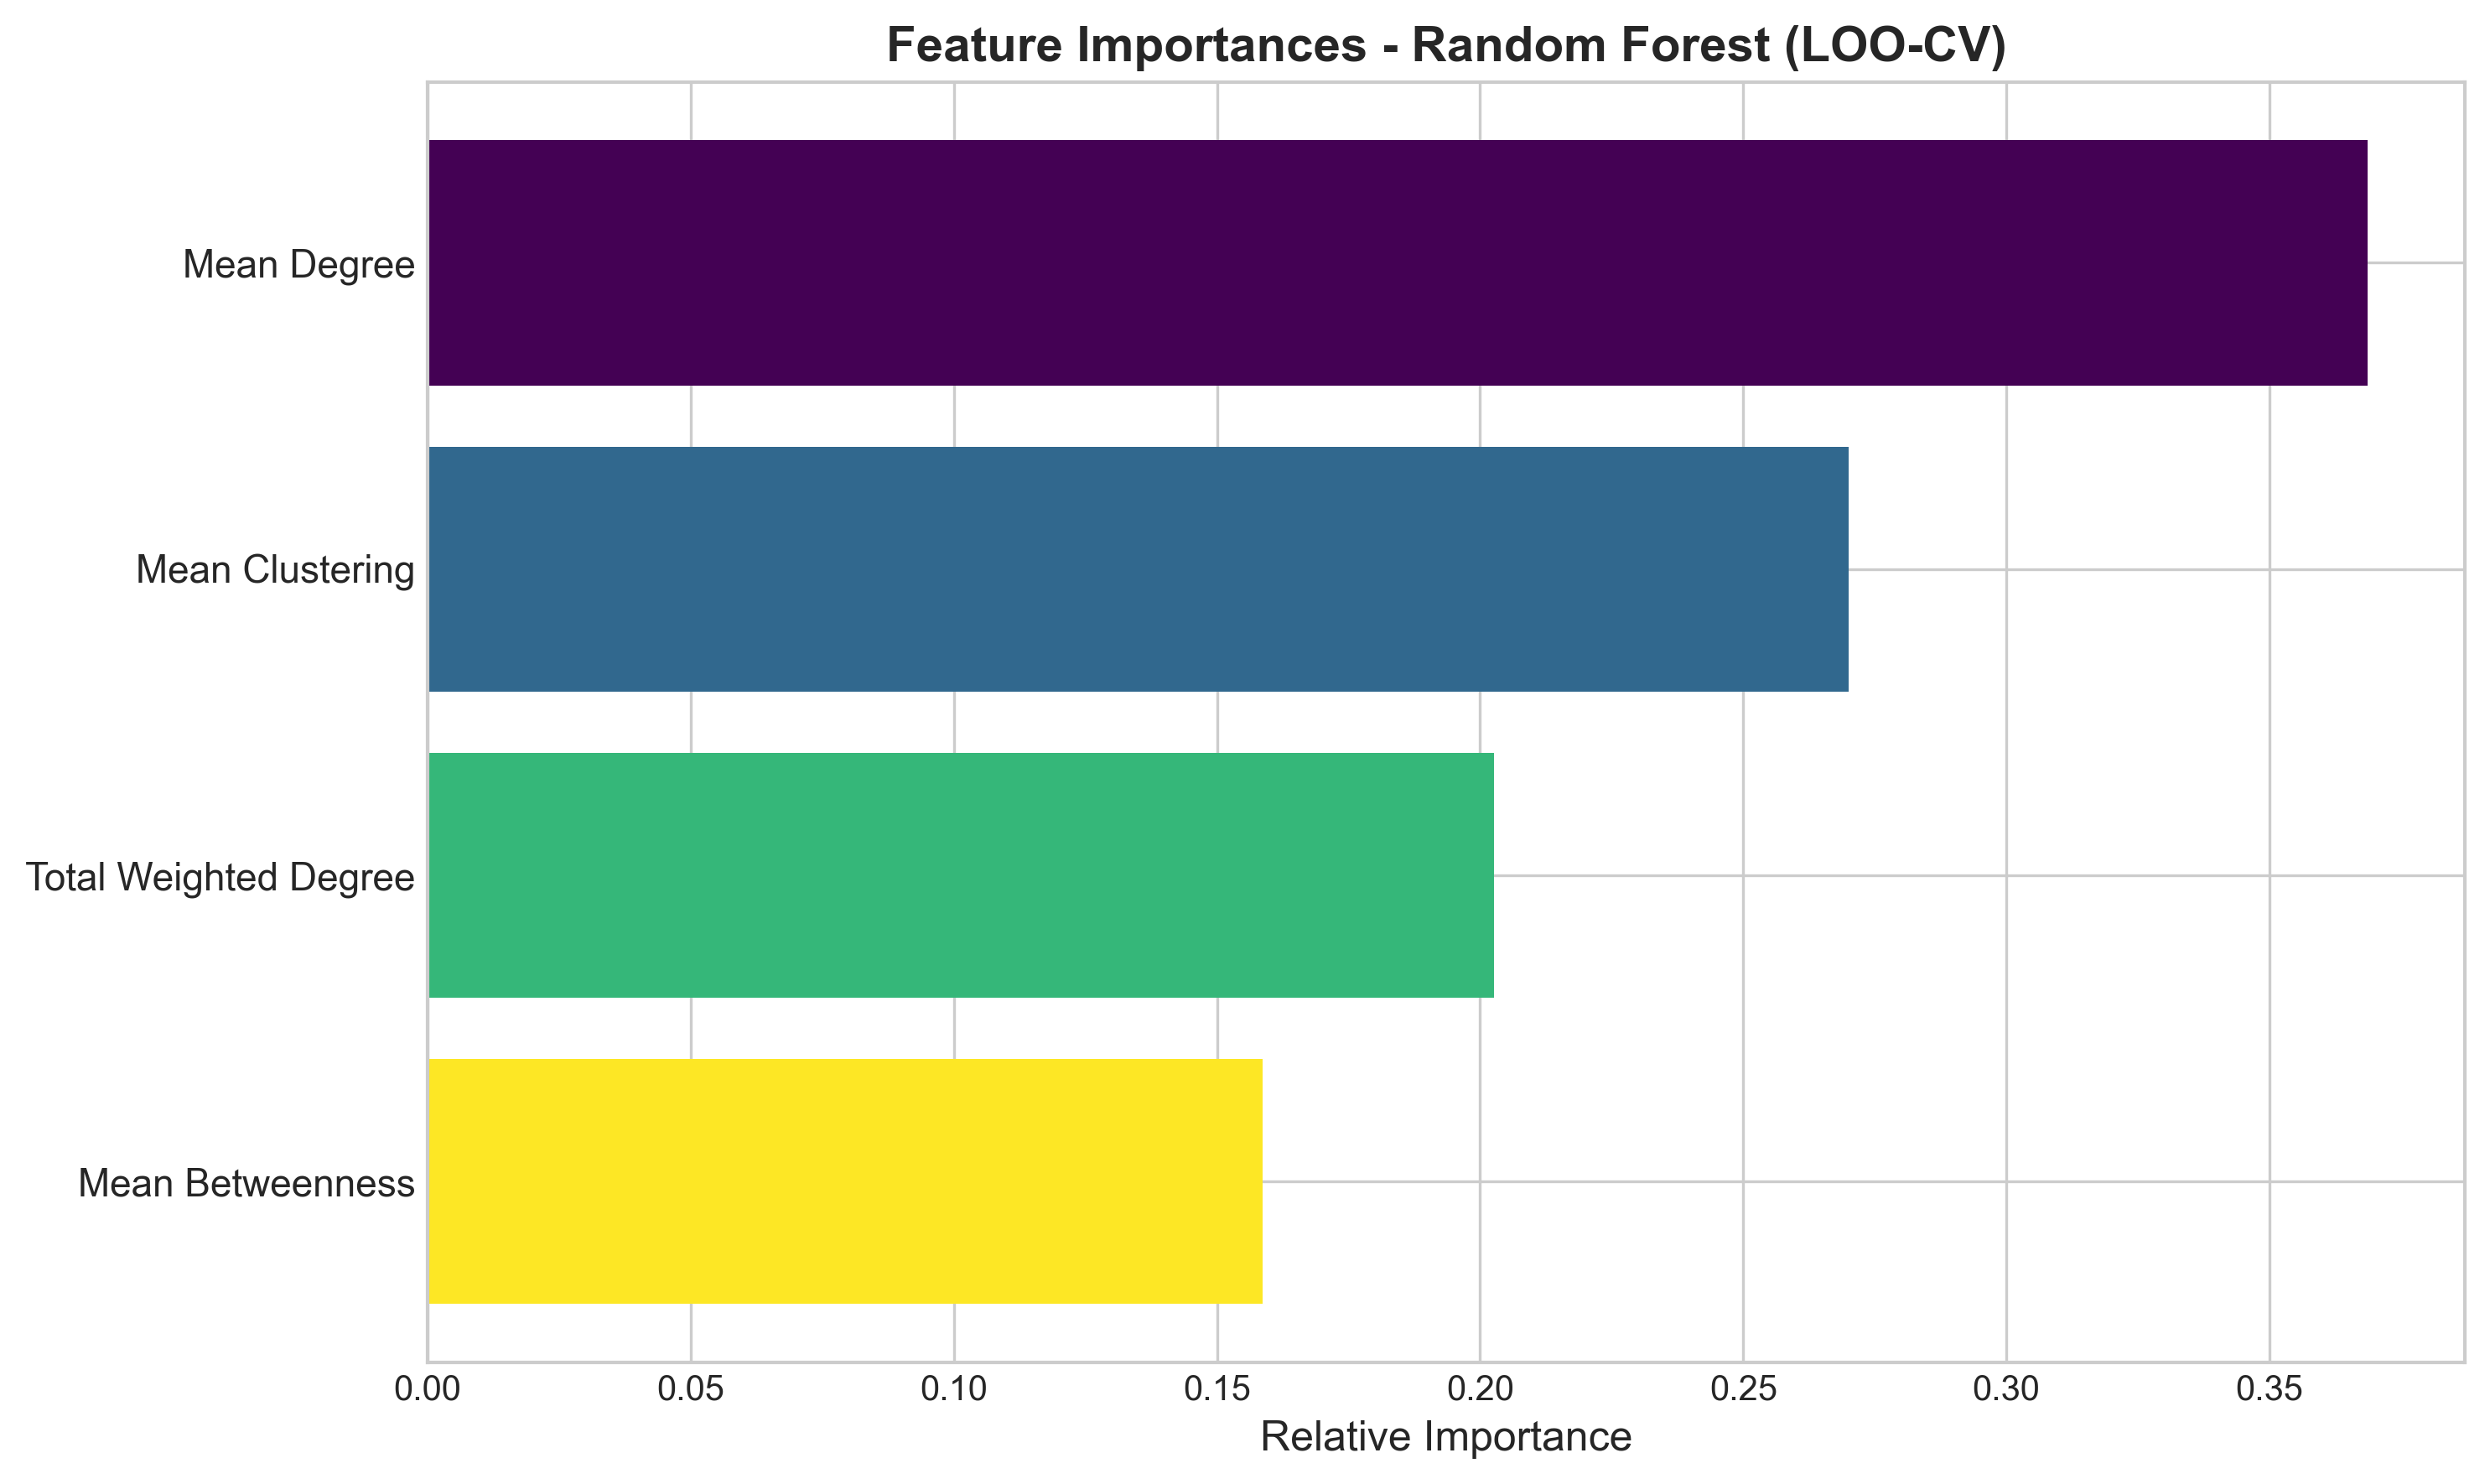
\includegraphics[width=0.98\linewidth]{feature_importances.png}
\caption{Importancias de las características del Random Forest.}
\label{fig:feature_importances}
\end{figure}

La importancia relativa de las variables fue:
\begin{itemize}[nosep,leftmargin=*]
    \item grado promedio: 0.369,
    \item clustering promedio: 0.270,
    \item suma de grado ponderado: 0.203,
    \item betweenness promedio: 0.159.
\end{itemize}

\begin{figure}[H]
\centering
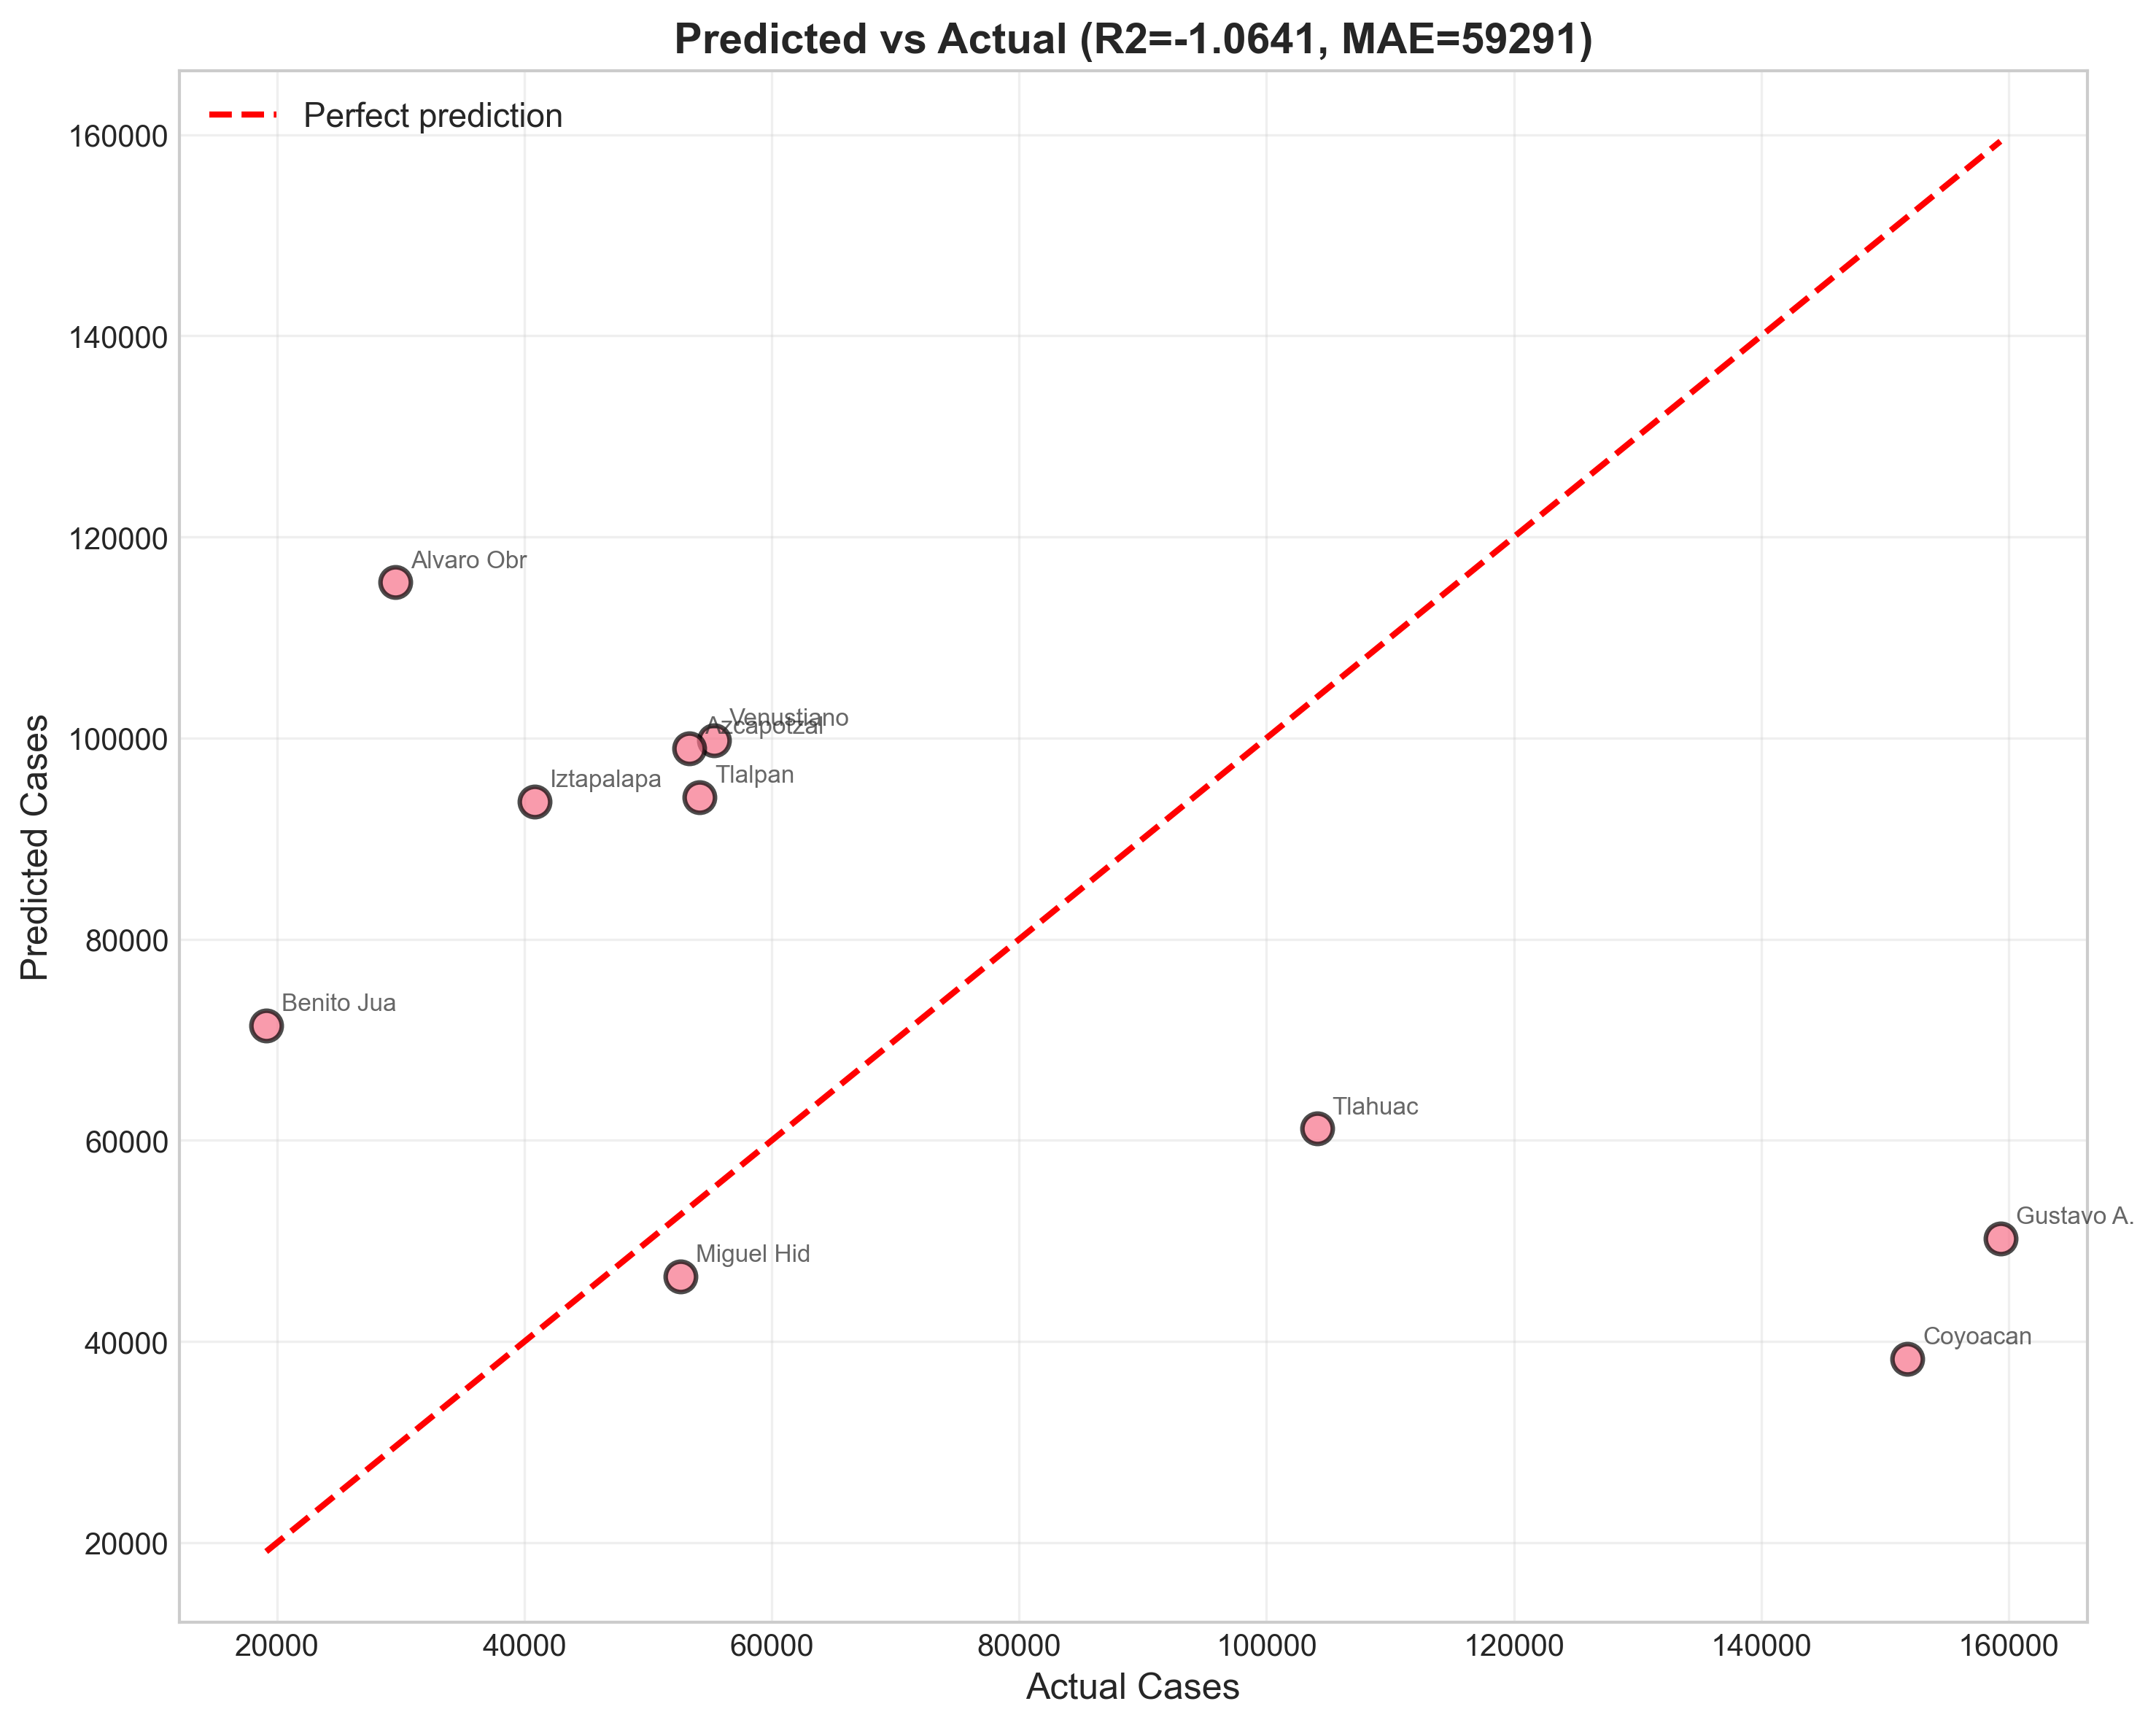
\includegraphics[width=0.98\linewidth]{predicho_vs_real.png}
\caption{Comparación entre los casos de COVID reales y los casos predichos por alcaldía.}
\label{fig:pred_real}
\end{figure}

La dispersión en Figura~\ref{fig:pred_real} ilustra que el ajuste no se concentra en torno a la diagonal de perfect prediction; varias alcaldías están sobregeneradas o subgeneradas, lo que evidencia la presencia de variables explicativas faltantes.

\section{Discusión}
Los resultados permiten extraer conclusiones sobre la influencia de la topología de la red del Metro en la propagación de enfermedades.

Primero, la red presenta una mezcla de conectividad y restricción. El alto clustering global sugiere zonas de fuerte interconexión local, mientras que el diámetro bajo indica la existencia de rutas cortas entre estaciones distantes. Esta combinación es típica de redes pequeño-mundo y es favorable para una difusión rápida de contagios.

Segundo, la comparación con redes sintéticas muestra que la red real es más conservadora que un grafo aleatorio o que una red de pequeño-mundo idealizada. Esta diferencia se debe a la geometría de las líneas, los transbordos localizados y los extremos terminales que actúan como amortiguadores.

Tercero, los resultados de aprendizaje automático enfatizan que la topología no es el único factor relevante. Un R$^{2}$ negativo indica que un modelo basado exclusivamente en métricas de red agrega poco valor predictivo frente a una constante. Es probable que la variación de casos entre alcaldías esté mediada por:
\begin{itemize}[nosep,leftmargin=*]
    \item densidad demográfica,
    \item condiciones socioeconómicas,
    \item ofertas de movilidad alterna,
    \item políticas locales de mitigación,
    \item uso de transporte privado.
\end{itemize}

\subsection{Aportes metodológicos}
Una contribución clave de este trabajo es la integración de datos de movilidad real (afluencia del Metro) con datos sanitarios oficiales y coordenadas geográficas de estaciones. Esto permite construir un modelo de red que no sólo refleja la conectividad física, sino también la intensidad de uso de cada nodo.

Además, la comparación con redes sintéticas provee un referente para interpretar los resultados: no basta con conocer el diámetro o el clustering, es necesario comparar contra estructuras alternativas para entender si una red es relativamente más o menos contagiosa.

\subsection{Implicaciones para salud pública}
Los hallazgos sugieren que las intervenciones en epidemias urbanas deberían priorizar las estaciones con alta betweenness y alto grado ponderado, ya que operan como puntos de concentración y paso de flujo. Estas estaciones son, por tanto, buenas candidatas para estrategias de mitigación dirigidas: control de aforos, ventilación reforzada, desinfección adicional y comunicación focalizada.

Sin embargo, la debilidad del modelo predictivo también indica que las políticas no deben basarse únicamente en la topología del Metro. Para ser efectivas, las intervenciones deben combinar información de red con datos socioeconómicos, epidemiológicos y de comportamiento.

\section{Conclusiones}
Este estudio demuestra que la red del Metro CDMX presenta características pequeño-mundo con alta agrupación local y distancias cortas. Las simulaciones SIR muestran que la red real genera un pico de infección menor que redes sintéticas aleatorias equivalentes, lo que indica un efecto amortiguador de la geometría física del sistema.

No obstante, la capacidad predictiva limitada del modelo de Random Forest revela que los casos de COVID-19 no pueden explicarse sólo con métricas topológicas agregadas. La recomendación metodológica es combinar modelos de red con covariables demográficas y de política pública para mejorar la explicación de la variabilidad espacial.

\section{Repositorio GitHub}

El código de este proyecto esta disponible y libre para su consulta en: \url{https://github.com/jossandoval/Proyecto-Final-Analisis-de-Redes-Sociales}

\bibliographystyle{plainnat}
\begin{thebibliography}{9}
\bibitem[Dirección General de Epidemiología(2020)]{dge2020}
Dirección General de Epidemiología, Secretaría de Salud de México. 2020-2021. \textit{Bases de datos abiertos COVID-19 México}. Recuperado de https://www.gob.mx/salud/documentos/datos-abiertos-bases-historicas-direccion-general-de-epidemiologia

\bibitem[Sistema de Transporte Colectivo(2020)]{metro2020}
Sistema de Transporte Colectivo, Gobierno de la Ciudad de México. 2020-2021. \textit{Afluencia diaria del Metro CDMX}. Portal de Datos Abiertos CDMX. Recuperado de https://datos.cdmx.gob.mx/dataset/afluencia-diaria-del-metro-cdmx

\bibitem[Mendoza Vega(2020)]{mendoza2020}
Mendoza Vega, J. B. 2020. \textit{Coordenadas del Metro CDMX} [conjunto de datos]. GitHub. Recuperado de https://github.com/jboscomendoza/coordenadas\_metro\_cdmx

\bibitem[Watts \& Strogatz(1998)]{watts1998collective}
D. J. Watts y S. H. Strogatz. 1998. Collective dynamics of small-world networks. \textit{Nature}, 393(6684):440--442.

\bibitem[Barabási \& Albert(1999)]{barabasi1999emergence}
A.-L. Barabási y R. Albert. 1999. Emergence of scaling in random networks. \textit{Science}, 286(5439):509--512.

\bibitem[Newman(2003)]{newman2003structure}
M. E. J. Newman. 2003. The structure and function of complex networks. \textit{SIAM Review}, 45(2):167--256.

\bibitem[Pastor-Satorras \& Vespignani(2001)]{pastor2001epidemic}
R. Pastor-Satorras y A. Vespignani. 2001. Epidemic spreading in scale-free networks. \textit{Physical Review Letters}, 86(14):3200--3203.

\bibitem[Cormack et al.(2009)]{Cormack2009ReciprocalRF}
G. V. Cormack, C. L. A. Clarke y S. Buettcher. 2009. Reciprocal rank fusion outperforms condorcet and individual rank learning methods. \textit{SIGIR}, pages 758--759.
\end{thebibliography}
\end{document}
